\begin{frame}{Oscilloscope}
    \begin{itemize}
        \item The core of the measurement setup for SCA is the oscilloscope. 
        \item It is a device that takes samples of the measured voltage signal over time.
        \item It can either be connected to the power supply of the DUT for power measurements or can measure electromagnetic (EM) signals through an EM probe.
        \item The main component of such an instrument is an analog-to-digital (ADC) converter, which takes the analog value of the measured signal (voltage, in our case) at the specified sampling rate, and changes it into a digital value.
        \item The precision of this value is generally between $8 - 12$ bits for mid-range oscilloscopes, and the sampling rate ranges from hundreds of mega samples per second (MS/s) to several giga samples per second (GS/s).
    \end{itemize}
\end{frame}

\begin{frame}{Oscilloscope measurement}
    \begin{itemize}
        \item When measuring analog signals, such as voltage, with digital devices, it is important to note that we are measuring a continuous value with equipment that \textit{samples} such a value at periodic intervals (called a \textit{time sample}) and stores it in a binary format with limited precision.
        \item Therefore, \textit{discretization} is applied twice -- first in the time domain, and then to the value itself.
        \item According to the Nyquist-Shannon sampling theorem, the sampling rate of the measurement device should be at least twice the highest frequency component of the measured signal.
        \item It is a good rule of thumb to have the oscilloscope sampling rate at least $4\times$ the target device frequency when doing measurements for power analysis attacks.
    \end{itemize}
\end{frame}

\begin{frame}{Sampling rate}
    \begin{figure}
    \centering
    \begin{tabular}{cc}
        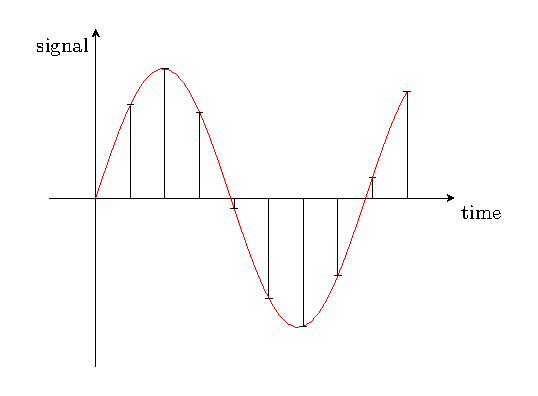
\includegraphics[width=0.45\textwidth]{fig/_TikZ__Digital_sine_book-2.pdf} & 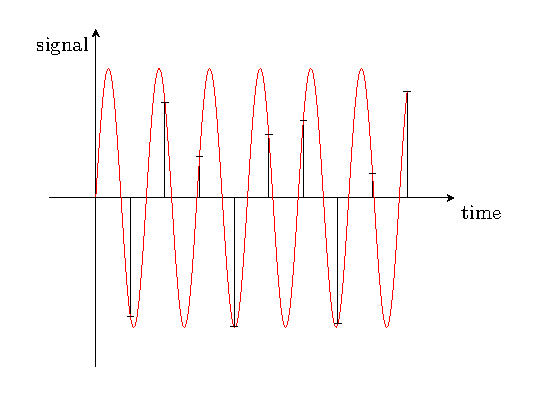
\includegraphics[width=0.45\textwidth]{fig/_TikZ__Digital_sine___high_freq_book-2.pdf} \\
        (a) & (b)
    \end{tabular}
    \caption{Digital sampling of a continuous signal with 10 samples of (a) low-frequency signal, (b) high-frequency signal.}
    \label{fig:sampling}
\end{figure}
\end{frame}

\begin{frame}{Attack setting}
    \begin{itemize}
        \item The precision of the oscilloscope specifies how many values can the sampled output value take, e.g., an 8-bit ADC would give a range of 256 values, which is sufficient for an SCA attack in most cases.
        \item An important task during the acquisition is capturing the correct time window corresponding to the operations we want to measure.
        \item In laboratory conditions, it is common to use an artificial trigger signal that indicates the start/end of the encryption.
        \item In real-world settings, it is necessary to identify the correct position by examining the captured signal -- this is usually done based on the evaluator's expertise.
    \end{itemize}
\end{frame}

\begin{frame}{Probes}
    \begin{itemize}
        \item Near-field electric and magnetic probes are an essential part of the setup when doing electromagnetic side-channel analysis.
        \item They can be connected to the oscilloscope in a passive way or with an amplifier.
        \item Optionally, a bandpass filter can be used to only pass the relevant frequencies and discard the rest.
        \item Several established companies, such as Riscure and Langer, provide probes suitable for EM SCA.
        \item Due to the simplicity of the probe design, researchers have also been building their own probes since the early days of SCA.
        \item Generally, a coiled copper wire is sufficient, with a coil diameter of at most a few hundred microns.
    \end{itemize}
\end{frame}